\documentclass[letterpaper,10pt, jcp, aps]{revtex4-1}
%\documentclass[superscriptaddress,pre,reprint,showpacs]{revtex4-1}

\usepackage[utf8]{inputenc}
\usepackage{amsmath, amsfonts}
\usepackage{graphicx}
\usepackage{natbib}
\usepackage{caption}
\usepackage{subcaption}
%\usepackage{authblk} parece ser que ya esta metido cuando usas preprint

\usepackage{hyperref}


%\bibliographystyle{alpha}

%opening

%\author{Rosa Rodríguez \& David P.~Sanders \& W. P. K. Zapfe}
%\affil{Departamento de Física, Facultad de Ciencias, Universidad Nacional Autónoma de México, Ciudad Universitaria, Del.~Coyoacán, México D.F. 04510, Mexico}

\usepackage{mathptmx}
% I dont know if that package is compatible with revtex.

\newcommand{\defeq}{:=}
\newcommand{\mean}[1]{\left \langle #1 \right \rangle}
\newcommand{\rd}[1]{\mathrm{d}{#1} \,}
\newcommand{\RR}{\mathbb{R}}
\newcommand{\vv}{\mathbf{v}}
\newcommand{\indicator}[1]{\mathbf{1}_{ \{   #1 \} } } 
\newcommand{\etal}{et al.\ } 

\setlength{\parskip}{10pt}
\setlength{\parindent}{0pt}


\begin{document}

\title{Exact hopping and collision times for two discs in a box}

\author{Rosa Rodríguez}
\email{rosa.g.asor@gmail.com }
\affiliation{Physics Department, McGill University}

\author{David P.~Sanders}
\email{dpsanders@ciencias.unam.mx}
\affiliation{Departamento de Física, Facultad de Ciencias, Universidad Nacional Autónoma de México}

\author{W.~P.~Karel Zapfe}
\email{karelz@fis.unam.mx}
\affiliation{CINVESTAV-IPN, Mexico}


\begin{abstract}
We study two the molecular dynamics of two discs bouncing within a rectangular box.
Using exact formulas from ergodic theory, applicable in a broad range of situations, we obtain exact expressions for mean hopping times, wall collision times and disk-disk collision times.
The only difficulty is in establishing the corresponding surface
of section and its measure.  
We compare the exact analytical results against Monte Carlo simulations, 
and also give numerical comparisons to first event times.
\end{abstract}

\maketitle



\section{Introduction}

%\typeout{`` this is ``  \the\columnwidth }

In statistical mechanics, distributions of collision times have played a fundamental role 
since Boltzmann REF, since properties
such as mixing, reaction and diffusion rates depend on them REFs.

For balls in a box, two fundamental events are \emph{hopping},
in which two particles interchange position along some
axis of interest, and \emph{collision} of the particles. 
A highly simplified model which has been successfully  used for
this research consists of two discs inside a rectangular
box \cite{Awazu01, Munakata02, Suh05}. The discs move rectilinearly until they undergo
elastic collisions either with a wall of the box, or with one another; this has been called ``inertial motion'' (to distinguish it from Brownian motion) REF, and can be thus be thought of as a billiard model REFs.

Previous work
by Bowles \etal gives general quantitative results for the mean hopping 
time for both inertial and Brownian dynamics \cite{Bowles04}. 
They use arguments from Transition State Theory 
to provide expressions for the general behavior of these quantities, as functions of the
radius of the discs. %Their results show the adequate algebraic behavior.
A great deal of work has expanded along that line  \cite{Suh05, Ball09}.
There is also a statistical thermodynamic treatment by Munakata \etal 
which deals very comprehensively with partition functions, pressure,
and temperatures \cite{Munakata02, Munakata06}. 

Our  primary goal in this paper is
to give  \emph{exact} results for mean hopping and collision times of two discs under 
inertial motion and compare them with first hopping and collision times.
Using a fundamental result from ergodic theory, e show that the former can 
be obtained  as a closed analytic expression dependent only
on the geometric parameters of the system, which turns 
out to be a rational function whose limiting form
has the algebraic exponent previously predicted REF, while
the latter follow closely the first, but with appreciable
qualitative differences. 

The exact treatment  turns to be  feasible because  
the reduced model is a hard sphere billiard REF.
Such systems are a widely-studied model in
statistical physics and nonlinear dynamics REF,
that have provided us with a deep mathematical understanding
about  the properties collectively called  \emph{Hard Chaos} 
(hyperbolicity, ergodicity and mixing qualities \cite{Sinai70, Gallavotti74}). 
One such system is the
gas of discs in a rectangular box \cite{SzaszBook00}, 
for which the simplest non-trivial
realization is the case of  two discs inside the box, our
present model.
This billiard is chaotic in a
strong sense \cite{Sim99}. The system  is thus amenable
to analytic treatment
and rigorous results have been obtained from ergodic theory \cite{MarkChern}.

%The previous  results on
%inertial dynamics can be extended  by particularizing 
%exact expressions for the mean return times (MRT). 
%We shall  obtain them through application of 
%Machta and Zwanzig formula for residence times \cite{MachtaZwan} ??
%We shall also  compare \emph{mean event times} with 
%\emph{mean first event times} (MFET),
%and give some arguments to explain the agreement between the two. 
%Brownian dynamics shall be discussed elsewhere \cite{WorkInProgress}.
%We shall also provide this paper with supplementary material 
%detailing the calculations. 



\section{Model: Two discs in a rectangular box}


% Voy a quitar todas las referenacias a la variable $d$ y el díametro
% nadamas nos están estorbando en las formulas y fastidiar al lector
% con una caracterización redundante del disco es mala onda.
We consider two discs of radius $r$  %(and diameter $d=2r$) 
in a box of width $w$ and height $h$ (see figure \ref{billar01}). 
The discs move inertially in the absence of forces, 
following straight line trajectories,
and undergo elastic collisions with each 
other and with the walls of the box.
We take the mass of each disk as unitary; the kinetic energy
is the value of the Hamiltonian function inside the billiard table:
\begin{equation}
H(q,p)=\frac{1}{2}(\|p_1\|^2+\|p_2\|^2)=1.
\end{equation}

\begin{figure}[h]
  \begin{center}
  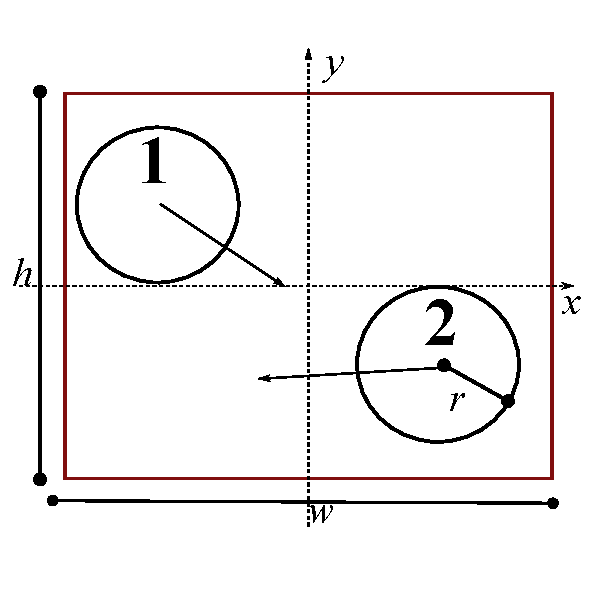
\includegraphics[width=0.40\textwidth]{FigurasPerfectas/DiscosenCajaCuadrada01.pdf}
  \end{center}
  \caption{The billiard and its parameters. Coordinates
    have their origin at the geometrical center of the 
    billiard table.}\label{billar01}
\end{figure}

We denote the position of the center of the $i$th disc by 
$(x_{i}, y_{i})$ for $i=1,2$. Since the discs are hard, 
the disc centers are restricted to the region 
$(x_i, y_i) \in [-a,a] \times [-b, b]$, where 
$a \defeq a(r) \defeq \frac{w}{2} - r $ and
$b \defeq b(r) \defeq \frac{h}{2} - r $.


The exclusion condition preventing the discs from overlapping is $(x_1-x_2)^2 + (y_1-y_2)^2 \ge (2r)^2$.
It is thus useful to perform an orthogonal change of coordinates (rotation) and work in terms of the new coordinates
\begin{equation}\label{cambiocoor01}
 x \defeq \frac{x_1 - x_2}{\sqrt{2}}; 
\quad X \defeq \frac{x_1 + x_2}{\sqrt{2}}; 
\quad y \defeq \frac{y_1 - y_2}{\sqrt{2}}; 
\quad Y \defeq \frac{y_1 + y_2}{\sqrt{2}}.
\end{equation}

%%This is WRONG, or better, is not precise enough.
In these coordinates, the configuration space is given by the following
intervals:
$x \in [-a \sqrt{2}, +a \sqrt{2}]$ with 
$X \in [-a \sqrt{2} + |x|, a \sqrt{2} - |x|]$; and 
 $y \in [-b \sqrt{2}, b \sqrt{2}]$ with $Y \in [-b \sqrt{2} + |y|, +b \sqrt{2} - |y|]$.
The non-overlapping constraint becomes $x^2 + y^2 \ge 2 r^2$.
The horizontal and vertical coordinates transform independently
from each other, and the Jacobian is in each case equal to $1$.

The constraints define a four-dimensional
rectangular prism, with a four-dimensional excluded cylinder inside.
This cylinder has radius $r\sqrt{2}$ and lies
in  a diagonal position along the axes $X, Y$.
The prism surface is the outer boundary of the configuration space,
while the cylinder is the excluded volume, and its surface
acts as a reflecting inner boundary.
The dynamics in this space follow
the usual billiard rules: free flight until
encounter with a wall, then elastic reflection.
The outer borders are flat, so the
hyperbolicity is due to the inner dispersing
boundary \cite{Sim99}, which represents the collision of
two discs in the original space.


\section{Mean time between events}


\subsection{Known facts on collision rates}

A system of $N$ hard spheres confined by hard walls in a $D$-dimensional
space may be treated as a billiard system 
in which a single point  particle undergoes free motion between reflecting obstacles 
in a $ (D N) $-dimensional configuration space \cite{Sinai70, Sim99, MarkChern}. 
If the resulting billiard is ergodic and hyperbolic, then we know that
these systems are equivalent to Bernoulli flows \cite{Gallavotti74}.
For such systems,an exponential decay of 
distributions \cite{AbadiGalves} with potentially
long algebraic tails \cite{ZasTip};
this includes recurrence times and
first encounter times. 

We also
have a result for the mean free time, i.e.\ the mean time between 
collisions of the particle with the walls \cite{MarkChern}. 
This can be thought of as a mean return time to the $(D-1)$-dimensional 
(i.e. co-dimension $1$) cross-section given by the wall boundaries.
The general formula for that time is REF
\begin{equation}\label{meanfreetime}
 \mean{\tau} = \frac{|Q|}{|A|} \frac{|S^{D-1}|}{|B^{D-1}|}.
\end{equation}
Here $|Q|$ denotes the $D$-dimensional volume of the available 
space in the billiard and 
$|A|$ the $(D-1)$-dimensional area of the cross-section.
 $|S^{D-1}|$ is the $(D-1)$-dimensional area of the unit sphere in $\RR^D$, given by
\begin{equation}
  |S^{D-1}| = \frac{2 \pi^{D/2}}{\Gamma(D/2)},
\end{equation}
where $\Gamma(\cdot)$ is the gamma function. 
$|B^{D-1}|$ is the volume of the unit ball 
in $\RR^{D-1}$, given by $|B^{D-1}| = |S^{D-2}| / (D-1)$.
In Equation~\eqref{meanfreetime},  the particle has 
its velocity scaled to unity.  USE GENERAL VALUE INSTEAD?

Machta and Zwanzig \cite{MachtaZwan} used a similar method to derive an escape 
time across a non-existent boundary by treating it as a recurrence time.
%Since it is an escape time, they used velocities whose components point only 
%perpendicularly to the ``exit wall''.
In our case, we are mainly interested in the mean return time to 
a co-dimension-$1$ cross section, 
which is defined by the exact moment
in which the disk interchange their horizontal position. This is simply
\begin{equation} \label{condchoque}
x_1 = x_2.
\end{equation}
We call such an event a ``hop''. Other first events shall also be studied
to test the robustness of the methods followed here.

Given that each disk has different momentum, but
they can interchange it without affecting the
total energy, we take into account the mass $m$ of each disk 
and the total kinetic energy $E$.
If both discs have the same mass then $\sum_i \vv_i^2 = 2E / m$.
The above result, as derived by Chernov, 
was for the case $\sum_i \vv_i^2 = 1$, or $m=1$ and $E=\frac{1}{2}$.  
For more general values of $E$ and $m$, 
we are simply working on a different energy surface in phase space. 
The particle trajectories are identical but the velocities differ
by a factor of
$\sqrt{2E/m}$. All times must divided by this value, 
giving for
the mean time between events the general formula:
\begin{equation} \label{meantimegeneral}
  \mean{\tau} =  \frac{1}{\sqrt{2E / m}} 
\frac{|Q| \, |S^3|} {|A| \, |B^3|}.	
\end{equation}
In our particular case, the effective dimension is four,
and $E=m=1$, so that the general factor of the formula appear as:
\begin{equation} \label{meantimegeneralredux}
   \frac{1}{\sqrt{2E / m}} 
\frac{|S^3|}{|B^3|}=\frac{3\pi}{2\sqrt{2}}.	 
\end{equation}

The next step is obtaining the Volume (4 dimensional measure) of
the available space and the Area (3 dimensional induced measure) of
the collision conditions. We devote the next section to
show the procedure, details can be found in the Appendix.


The general result is
\begin{equation}
 \mean{\tau} = \frac{|Q|}{|A|} \frac{|S^{d-1}|}{|B^{d-1}|}
\end{equation}
when the particle has velocity $1$.
Here, $|Q|$ denotes the $d$-dimensional volume of the available space in the billard and $|A|$ the $(d-1)$-dimensional volume of the cross-section.
 $|S^{d-1}|$ is the $(d-1)$-dimensional volume of the unit sphere in $\RR^d$, given by
\begin{equation}
  |S^{d-1}| = \frac{2 \pi^{d/2}}{\Gamma(d/2)},
\end{equation}
where $\Gamma(\cdot)$ is the gamma function. $|B^{d-1}|$ is the volume of the unit ball in $\RR^{d-1}$, given by $|B^{d-1}| = |S^{d-2}| / (d-1)$.

The system of two hard discs is equivalent to a billiard in $d=4$ dimensions, so that
\begin{equation}
 |S^{d-1}| = |S^3| = 2 \pi^2; \qquad |B^{d-1}| = 4 \pi / 3.
\end{equation}


\section{Calculation of Volumes and Areas}

The configuration
space is an four dimensional prism with a four dimensional
cylinder subtracted.
The calculation can be carried out indirectly,
 using indicator functions for the
available space or for the prohibited space.

\subsection{Volume of available space}

We shall present the total four-dimensional volume as a product integral
of all available positions. To grasp the idea, a 
diagram is shown in Figure \ref{diagintegra01}. Our
principal integral is the available free $4D$ volume, which 
we shall denote $V_\text{free}$:
\begin{multline}\label{volindic}
 V_\text{free} = \\ \int\limits_{x_1 = -a}^a \rd x_1 \int\limits_{x_2 = -a}^a \rd x_2 
\int\limits_{y_1 = -b}^b \rd y_1 \int\limits_{y_2 = -b}^b \rd y_2 \, \indicator{ (x_1-x_2)^2 + (y_1-y_2)^2 \ge (2r)^2 },
\end{multline}
where $\indicator{Z}$ indicates the indicator function of the set $Z$, 
given by $\mathbf{1}_Z (x) = 1$ if $x \in Z$, and $=0$ if $x \notin Z$, 
which restricts the integral to the desired region $Z$.
\begin{figure}[h]
  \begin{center}
    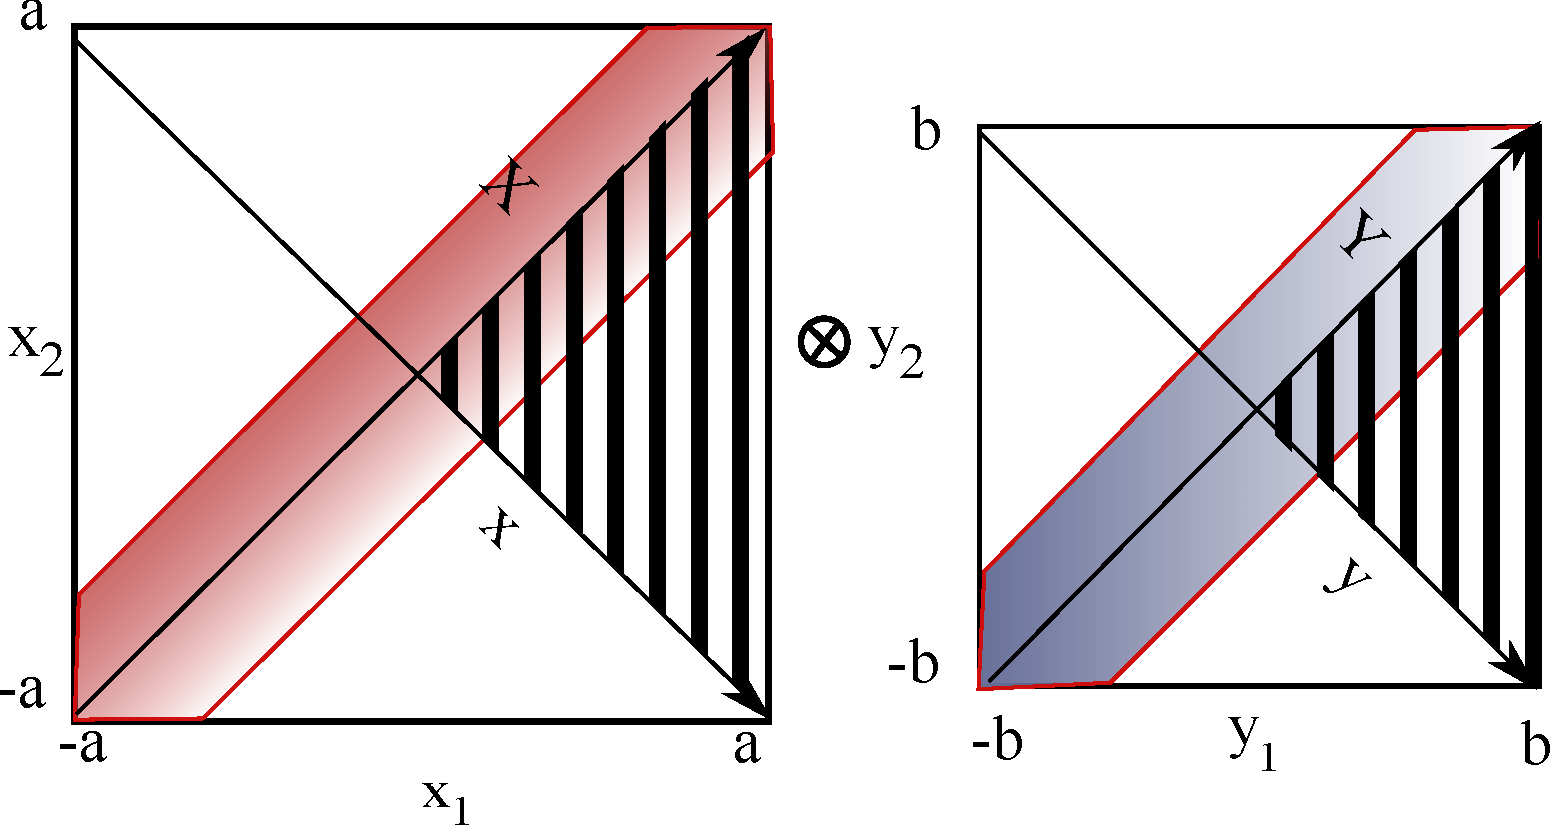
\includegraphics[width=0.45\textwidth]{FigurasPerfectas/diagramintegra01.pdf}
  \end{center}
  \caption{The space to integrate is the product of the subspaces
    belonging to horizontal and vertical coordinates. The colour
    bands represents the ``exclusion'' set, where the condition 
    $ (x_1-x_2)^2 + (y_1-y_2)^2 \ge d^2 $ is not met. 
    The width of each band is dependent on the particular 
    point of evaluation
    on the \emph{other} subspace. The diagonal coordinates
    make the expression to evaluate simpler. Due to 
    symmetry, we only evaluate the area in stripes and
    multiply the result by 16.}\label{diagintegra01}  
\end{figure}

It is easier to represent the  
excluded cylinder in the coordinates defined in 
the set of equations \ref{cambiocoor01}. Then the exclusion condition
is orthogonal to the coordinates $X,Y$ and they do not appear
on the indicator function. 
\begin{multline}\label{integraltotal}
 V_\text{free} = \\ \int\limits_{x=-a \sqrt{2}}^{a \sqrt{2}} \rd x 
\int\limits_{X=-a \sqrt{2} + |x| }^{a \sqrt{2} - |x|}  \rd X
 \int\limits_{y=-b \sqrt{2}}^{b \sqrt{2}} \rd y
\int\limits_{Y=-b \sqrt{2} + |y| }^{b \sqrt{2}-|y|}  \rd Y
\, \indicator{ x^2 + y^2 \ge 2r^2  }.
\end{multline}
In these coordinates, $X$ and $Y$ do not appear in the function to be
integrated, 
so that these integrals may be done trivially. After that we are left 
with the  following two-dimensional integral:
\begin{multline}
 V_\text{free}  = \\ \int\limits_{x=-a \sqrt{2}}^{a \sqrt{2}} \rd x  \int\limits_{y=-b \sqrt{2}}^{b \sqrt{2}} \rd y
2 \left( a \sqrt{2} - |x| \right) \, 2 \left( b \sqrt{2} - |y| \right) \indicator{ x^2 + y^2 \ge 2r^2 } \\
 = 16 \int\limits_{x=0}^{a \sqrt{2}} \rd x  \int\limits_{y=0}^{b \sqrt{2}} \rd y 
\left( a \sqrt{2} - x \right) \left( b \sqrt{2} - y \right) \indicator{ x^2 + y^2 \ge 2r^2 },
\end{multline}
where we used the symmetry indicated in the figure \ref{diagintegra01}.
Thus $V_\text{free} = 16(I_1 + I_2)$, where $I_1$ is the region where the value of $y$
is affected by the exclusion condition and $I_2$ is where it is not affected
by it. 
We have
\begin{align}
 I_1 &= \int\limits_{x=0}^{r\sqrt{2}} \rd x \int\limits_{y = \sqrt{ 2r^2 - x^2}}^{b \sqrt{2}} \rd y
\left( b \sqrt{2} - y \right)  \left( a \sqrt{2} - x \right) \\
&= 	
2 a b^{2} r  + \textstyle \frac{1}{6} (a+b) (2r)^{3} - \frac{1}{32}  (2r)^{4} - \frac{1}{4} {\left(\pi a b + b^{2}\right)} (2r)^2,
\end{align}
and
\begin{align}
 I_2 &= \int\limits_{x=r  \sqrt{2}}^{a \sqrt{2}} \rd x  \int\limits_{y = 0}^{b \sqrt{2}} \rd y
 \left( b \sqrt{2} - y \right)  \left( a \sqrt{2} - x \right)  \\
&=	
{\left( a^{2} - 2ar +   r^{2}\right)} b^{2}.
\end{align}
Thus 
\begin{align}\label{volumeabd}
 V_\text{free}
 & =  16 a^{2} b^{2}  - 16 \pi a b r^{2} + \textstyle \frac{64}{3} (a+b) r^{3}  - 8 r^{4} \\
&= V_\text{prism} - V_\text{cyl},
\end{align}
as was previously obtained by Munakata and Hu \cite{Munakata02}.
For clarity we have divided this expression in the volume of the prism 
$V_\text{prism}=16 a^2 b^2$, and  the volume excluded by the overlapping
condition, denoted here by 
$V_\text{cyl}=  16 \pi a b r^{2} - \textstyle \frac{64}{3} (a+b) r^{3}  + 8 r^{4}$.

The substitutions $a\rightarrow (w-2r)/2$ and $b\rightarrow (h-2r)/2$ give us
 the volume as a function of the radius, for fixed table size:
\begin{multline}\label{volumewhd}
 V_\text{free} 
= (w-2r)^{2} (h-2r)^{2}  - \\ 
 \pi (w-2r)(h-2r) 4 r^{2} + 
\textstyle \frac{32}{3} (w+h-2r) r^{3}  
- 8^{4},
\end{multline}

%%Okey, tal vez esto no viene aqui al caso
There is a quirk in the above formula:
this is the available volume for the case when both
vertical and horizontal hopping are possible.
If we want to obtain the volume for all possible configurations
given $w,h,r$ ,
we also have to take into account the cases in which hopping is no
longer possible. 
We tacitly made the assumption that $h,w>4r$.  This affected our 
integration limits for the $X,Y$ variables in the step in eq. \ref{integraltotal}. 
A full discussion of the formula for the case in which either
$w$ or $h$ are smaller than $4r$ but there is still space for
the discs is discussed in \ref{app:area_volume}.

As an example, we consider the case where vertical hopping is possible
and horizontal is excluded,  $w \geq h$.
This case is divided into two sub-cases: if
$ h \leq  w < 2 h $ there is a value for $r$ for which hopping is not possible,
but the discs still fit inside. For $ 2 h \leq w $, vertical hopping is
possible until $ 2 r= h$ (where vertical movement is impossible). These cases
can be thought of as the configuration space becoming disjoint, and
some of the cross section areas staying outside it. Thanks to the symmetry of
the problem, in many cases the cross-section areas and 
volumes become disjoint components sharing the same fraction of
the total volume, making the transition smooth.

We cite the  result for $h/4  <r< w/4$ for illustrative purposes.
For readability we define another auxiliary variable,
$c=\sqrt{4r^2-b^2}$:
\begin{multline}\label{VolumenCasoFeo}
V_{h/4<r<w/4} = 32abr^2[\arccos(b/2r)-\arccos(a/2r))]\\
+\frac{64 r^3}{3 }[a((b-a)/2r)-b(c/2r+\sqrt{4r^2-a^2}/2r)]\\
-2r^2 (b^2-a^2)\\ 
+16[ a b^2 c (4\sqrt{2}-1-\sqrt{2}/3)
+c^2b^2 (\sqrt{2}/3-1) \big]
\end{multline}
In the case that $r$ is larger than both $h/4, w/4$, one must take
into account a similar
contribution which inverts the roles of $a$ and $b$. Then there is
a case where hopping is impossible. 

In order to not to pick a degenerate case for our numerical simulations,
we have set $w=1.5, h=1$. This covers all of the uses of the general volume formulas.


We have checked this result with simple Monte Carlo simulations, 
by generating random positions for the discs centers in 
$[-a,a] \times [-b,b]$ uniformly and 
counting the proportion of such initial conditions for 
which the two discs overlap. The fraction of these points to the 
total should give the fraction of prohibited volume over the hypercube
volume. The results are shown in the figure \ref{VolMonteC}.

\begin{figure}[h]
\centering
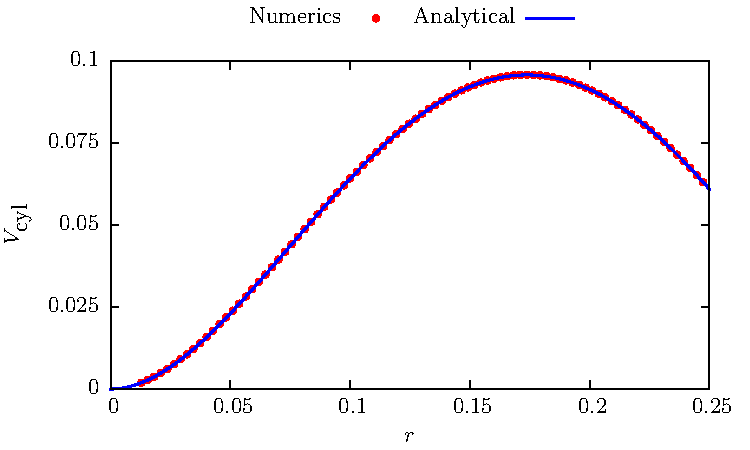
\includegraphics[width=0.45\textwidth]{./FigurasPerfectas/VolCyl02.pdf}
\caption{Formula for $V_\text{cyl}$, the area of the exclusion cylinder, compared
  against the numerics, from eq. \ref{volumeabd}.
  \pmb{esta es la grafica antigua, no el caso mas general}
}%\label{VolMonteC}%% 
\end{figure}

\begin{figure}[h]
\centering
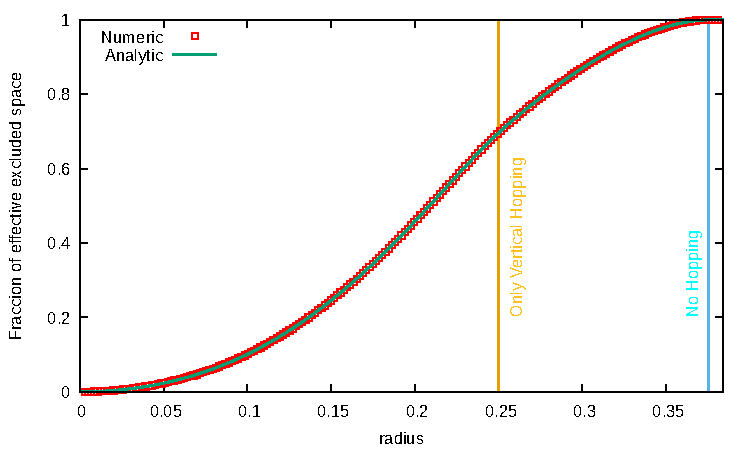
\includegraphics[width=0.45\textwidth]{./FigurasPerfectas/VolumenExacto01.pdf}
\caption{Formula for $V_\text{cyl}/V_\text{prism}$, the fraction of volume excluded from
  the avaible free volume.
  against the numerics, from eq. \ref{volumeabd}.
  \pmb{esta es el caso general. Esto también hay que hacerlo con las areas y así. }
}\label{VolMonteC}%% 
\end{figure}


The following subsections shall only show the formulas for $r<w/4, h/4$.
Bear in mind that some of the dynamics are possible above this limit,
it is only the position interchange that gets excluded. \\

%%
%% ¿Que ondas David, hacemos las simulaciones para el caso espantoso tambien?
%% Ok. Ya las voy haciendo


\subsection{Area of cross-section for
 vertical interchange (hops)}\label{areahop}

Our cross section ``areas'' are three dimensional manifolds
defined by relative simple equations. We shall denote their
measure by $A$.
The hopping cross-section 
$ \{y_1 = y_2\}$ becomes 
$\{ \sqrt{2}y=0 \}$ in the new coordinates.
For obtaining the measure,
we proceeded as follows:
First we concentrate the measure indicated on the eq. \ref{volindic}
multiplying by a Dirac Delta $\delta(y_1-y_2)$ on the integrating part
(for the adequate treatment of this Dirac Delta see the supplementary 
material \footnote{Appendix B: On the change of coordinates with Dirac Delta 
Operators. If your name happens to be David Sanders, then read it VERY slowly.}):
\begin{widetext}
\begin{equation}
 A_\text{hopp} = \int\limits_{x_1 = -a}^a \rd x_1 \int\limits_{x_2 = -a}^a \rd x_2 
\int\limits_{y_1 = -b}^b \rd y_1 \int\limits_{y_2 = -b}^b \rd y_2 \, \indicator{ (x_1-x_2)^2 + (y_1-y_2)^2 \ge (2r)^2 } \delta(y_1-y_2).
\end{equation}
\end{widetext}
Except for a factor $1/\sqrt{2}$ due to the change of variables
with the Dirac Delta, everything procedes as before. The integration is
simpler than in the other cases and results in 
\begin{equation}
 A_\text{hopp}  =  16 b(a-r)^2
\end{equation}
As before, the formula stops being valid for $r>w/4$. This time it has
no extention, as vertical hopping becomes impossible for a larger radius,
but it needs no correction for the exclusion of horizontal hopping. 

We made numericall simulations of the initial conditions for
veryfying these results. In this case we 
by counted the proportion of successful placements of hard discs 
for which the distance 
$|y_1 - y_2|$ was within a small tolerance of $0$. 
Results are shown in figure \ref{AreaHopp01}.

\begin{figure}[h]
\centering
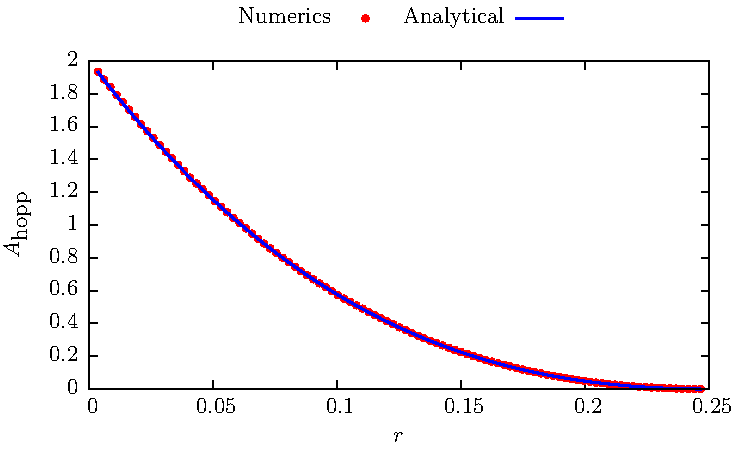
\includegraphics[width=0.45\textwidth]{./FigurasPerfectas/AreaHop02.pdf}
\caption{The hopping area, $A_\text{hop}$, 
  indicated in the formula in eq. \ref{AreaH}. As explained
in the text, it gives nonsense for $r>1/4$, but numerical values stay
exactly at zero, the correct value. } 
\label{AreaHopp01}
\end{figure}


\subsection{Area of cross section for collisions}

The area which represents collisions between the two discs is the cylinder area. 
This can be deduced in a similar manner to the free volume, shown in the last
section, or as the derivative of this formula, taking it as as a function evaluated at 
$r\sqrt{2}$. The calculation must be done taking $a,b$ as constants, so that
we do not obtain also the (negative) contribution for the flat ends of
the wedge at the cylinder's end. For the case $r<w/4$ the resulting area is:
\begin{align}\label{AreaChoque}
A_\text{collision} & =  
16\pi a b r -32 (a+b)r^2 +16 r^3 
\end{align}

We proceed in the same manner as last section, checking numerically which
random
conditions fall at a small tolerance of $0$ from the Collision Condition, and
plotting this as a fraction of the total volume. The result is shown in the
figure \ref{AreaChoqueTeoyNum}. 
\begin{figure}
\centering
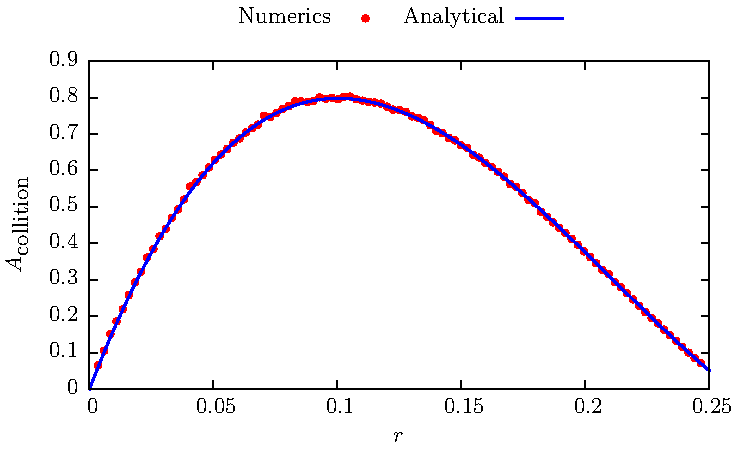
\includegraphics[width=0.45\textwidth]{./FigurasPerfectas/AreaCol02.pdf}
\caption{The numerical and theoretical calculation for the Area of the cross section
for collision between the discs.  The theoretical formula 
\ref{AreaChoque} breaks down at
$r>1/4$.}
\label{AreaChoqueTeoyNum}.
\end{figure}


\subsection{Area of cross section for  impacts on walls}

For comparison, we shall use also other area to compare
some properties of the decay of time distributions. The most natural choice
would be the mean time between any impact on the walls. This corresponds
to the adequate measure of the border of the four dimensional
billiard in which the dynamics takes place. This area is
the sum of the areas of the border of the
prism, taking into consideration the excluded tips of the cylinder. 
It shall be enough to calculate the cross section area for
the impact of one specific disk unto one specific wall and,
by means of the symmetry of the expressions, obtaining the whole
area. We proceed then to calculate the cross section corresponding to 
the disk labeled $1$ hitting the right wall. We accomplish that by
evaluating the next expression in a similar way to
the procedure carried out in section \ref{areahop}:
\begin{equation}\label{areaindic}
 A_{x_1+} =  \int_{x_2 = -a}^a \rd x_2 
\int_{y_1 = -b}^b \rd y_1 \int_{y_2 = -b}^b \rd y_2 \, \indicator{ (a-x_2)^2 + (y_1-y_2)^2 \ge 4 r^2 }
\end{equation}
The integration procedure is equally tedious, but
straightforward, the result is 
\begin{align}\label{areax1p}
 A_{x_1+} & = 8 a b^2-4  \pi b r^2 +\frac{16}{3}r^3 
 % & = 2(w-d)^2 (h-2)^2- \frac{\pi}{2} (h-d) d^2 +\frac{2}{3}d^3 
\end{align}
Once again, a simple Monte Carlo procedure verifies this result,
shown in fig \ref{area1derecha}. 

\begin{figure}
\centering
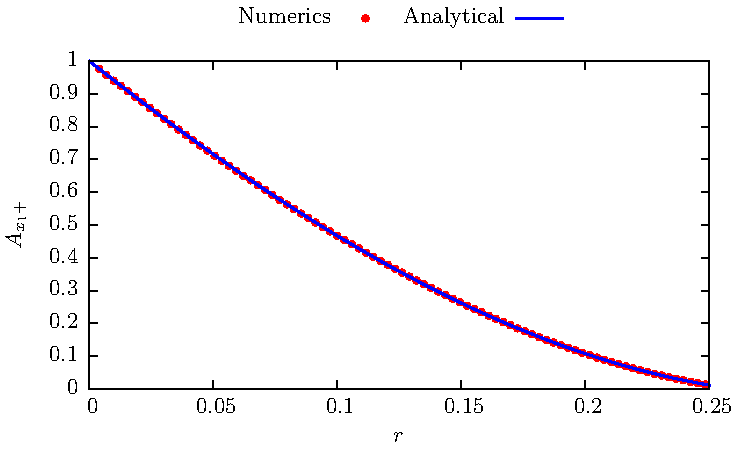
\includegraphics[width=0.45\textwidth]{./FigurasPerfectas/AreaParedx1Positiva02.pdf}
\caption{The numerical and theoretical calculation for the cross section area
for the impact of a determined disk with the right wall, as in eq. \ref{areaindic}.
Again, the formula stops being valid at $r>1/4$. }
\label{area1derecha}.
\end{figure}

Given into account the symmetry of the expression for either of 
the disk bouncing in each of the vertical walls, the
cross section area for this event is four times $A_{x_1+}$. On
the other hand, each bounce against the horizontal walls would
define a similar quantity, but with the roles of $a$ and $b$ switched.
The cross section area for any impact on the walls would then be:
\begin{align}\label{areawalls}
 A_\text{walls} & = 32 a b (a+b)-16 \pi r^2 (a+b) +\frac{128}{3}r^3 
 %&=  4 (w-d) (h-d)  (w+h-2d) -2 \pi d^2 (w + h-2 d) +\frac{16}{3}d^3. 
\end{align}
The cross section area for any impact or collision 
would be  the sum of the last expression
and the area for collisions between discs, in eq. \ref{AreaChoque}.


\section{Mean times between events}

In this section, we give exact results for the mean inter-event times for hopping, disc-disc collisions and disc-wall collisions.

%The three formulas have been checadas entre ellas y con gnuplot
% y la numerica: no aparecen factores espurios de raiz de dos
\subsection{Mean hopping time}

Inserting the results of the previous section 
into the formula for the mean times for crossing
surfaces of section, eq. \ref{meantimegeneral}, gives the times for 
horizontal hopping, 
collision between discs and impacts in general. For horizontal
hops we have:
\begin{equation}\label{hoptau}
 \mean{\tau_\text{hop}} = 	
\frac{3 \pi}{2\sqrt{2}}
\frac{2 a^{2} b^{2}  - 2 \pi a b r^{2} + \textstyle \frac{a+b}{3}  (2r)^{3}  -  r^4}
{ a \sqrt{2}  ( b - r )^2}.
\end{equation}
The limiting form for small discs is revealing: a constant
that depends only on the width of the table, since then the discs have almost no interaction:
\begin{equation}\label{hoptaulimit}
 \mean{\tau_\text{hop}} \overset{r \to 0}{\sim}
\frac{3 \pi}{4}w.
%%Esta ya la cheque con la numerica y esta PERFECTA, segun gnuplot y todos los 
%%Scripts
\end{equation}
Also of interest is the limit $r\sim a/4$, where hopping becomes
impossible. The lower term goes to zero as $r^2$ become approximately constant.
This agrees with heuristic arguments. 
In the particular case $w=h$ as in our examples,
setting $r=h/4-\epsilon$ gives the limiting behaviour 
\begin{equation}
 \mean{\tau_\text{hop}}(\epsilon) \overset{\epsilon \to 0}{\sim}
\frac{3 \pi}{8}
\frac{(1-\frac{2\pi+1}{32})}
{ \epsilon^2} w^3
\end{equation} 
This last expression coincides with that of Bowles et al. \cite[Equation~12]{Bowles04},
which
predicts the same exponent for the behaviour of this hopping time. The figures
2 and 4 of their article correspond to that regime. 

\subsection{Mean collision time}

For collisions between discs, we have, for the case $r<w/4$,
\begin{equation}\label{colltau}
 \mean{\tau_\text{coll}} = 	
\frac{3 \pi}{2\sqrt{2}}
\frac {2 a^{2} b^{2}  - 2 \pi a b r^{2} + \textstyle \frac{a+b}{3}  (2r)^{3}  -  r^4}
{2\pi a b r -4(a+b)r^2+2r^3}
\end{equation}
As expected, this goes to infinity with very small radius, its behaviour
approaching the expression
\begin{equation}\label{colltaulim0}
\mean{\tau_\text{coll}} \overset{r \to 0}{\sim}
\frac{3}{8\sqrt{2}}\frac{wh}{r}
\end{equation}
For the case in which the discs narrowly fit inside the table we need to
use the more cumbersome expression in eq. \ref{VolumenCasoFeo} and
the corresponding area. The time between collisions should go to zero.


\subsection{Mean wall impact time}

Lastly, for impacts on any of the walls we have obtained: 
\begin{equation}\label{impactwall}
 \mean{\tau_\text{wall}} = 	
\frac{3 \pi}{2\sqrt{2}}
\frac { 2a^{2} b^{2}  -  2\pi a b r^{2} + \frac{a+b}{3}(2r)^3 - r^4}
{4ab(a+b)-2\pi(a+b) r^2 + \frac{16}{3} r^3 }.
\end{equation}

Adding the areas representing the impact on the walls and
the collisions on the discs, we  obtain
the expression for \emph{any} 
collision in the system:
\begin{equation}\label{impactany}
 \mean{\tau_\text{any}} = 	
\frac{3 \pi}{2\sqrt{2}}
\frac { 2a^{2} b^{2}  -  2\pi a b r^{2} + \frac{a+b}{3}(2r)^3 - r^4}
{4ab(a+b)+2 \pi \sqrt{2} abr-(2\pi+4\sqrt{2})(a+b)r^2+(\frac{16}{3}+2\sqrt{2})r^3}.
\end{equation}

In the limit $r\rightarrow 0$ this is asymptotic to $3 \pi (hw)/(8\sqrt{2}(h+w))$.
This should correspond to the average impact time on the walls
for non-interacting point particles.
%but, then, such as system would not be chaotic and the limit is senseless.
%On the other hand, for the limit of radius as large as possible, we shall
%again use the extended expressions in the formula for volume and area.


\section{Comparison with numerics}

In this section, we compare the analytical results obtained with Monte Carlo simulations of the available volume and areas. To carry out these simulations, we ....

\subsection{Mean times for events}

We proceed to test last section formulas with
extensive numerical simulations.
The next three figures, \ref{MeanHopp01}, \ref{MeanCol01}, and \ref{MeanImp01},  
we compare the
numerical and analytically curves for the mean return times of different events.

\begin{figure}[h]
  \centering
  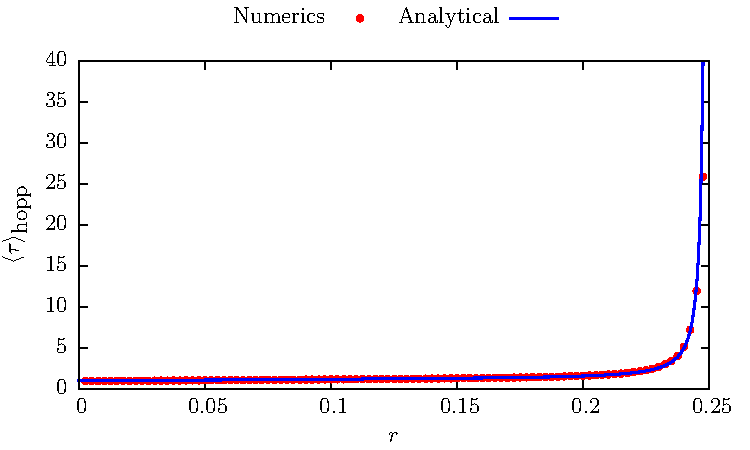
\includegraphics[width=0.45\textwidth]{./FigurasPerfectas/HopTimes02.pdf}
  \caption{The mean hopping time as function of the radius, Energy, mass, 
and geometry fixed, numeric and Analytic results.}\label{MeanHopp01}
\end{figure}

\begin{figure}[h]
  \centering
  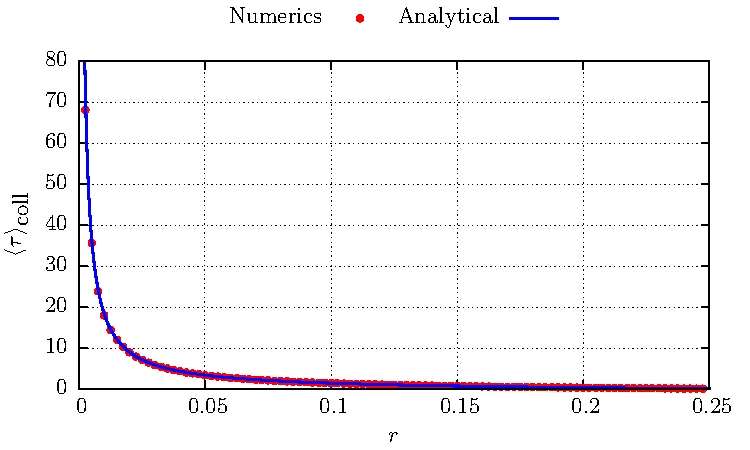
\includegraphics[width=0.45\textwidth]{./FigurasPerfectas/CollitionTimes02.pdf}
  \caption{The mean collision time as function of the radius. Same
    specifications as the last figure. }\label{MeanCol01}
\end{figure}


\begin{figure}[h]
  \centering
  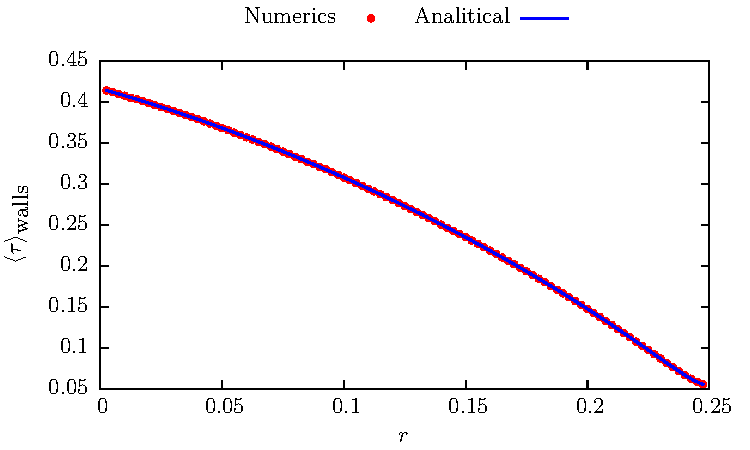
\includegraphics[width=0.45\textwidth]{./FigurasPerfectas/ImpactWall02.pdf}
  \caption{The mean impact-on-walls time as function of the radius. Again, same
    notes as the figure \ref{MeanHopp01}}\label{MeanImp01}.
\end{figure}

\pmb{Shall we plot the distributions for fixed interesting r? }

\section{Mean first event times}

Although we do not have a formula for the mean first event time as
we have for the mean return times, we can, with a slight modification
of our code, investigate the behaviour for these quantities. We have 
an interesting result: most \emph{first event times} deviate very slightly,
although systematically, from the \emph{mean return times}.

%This could be explained as follows:
%In an ergodic regime we could simply average over a sufficiently large
%sample of initial conditions instead of following each trajectory
%and sampling events along it. This means that the mean return time
%coincides with the mean first return time for large enough samples.
%A \emph{mean first event time} could be though of a \emph{mean
%first return time} with erroneous initial conditions, as if the
%trajectories had started, so there would be an \emph{average offset}
%for the times. As we show numerically, this is indeed the case. 


\begin{figure}[h]
  \centering
  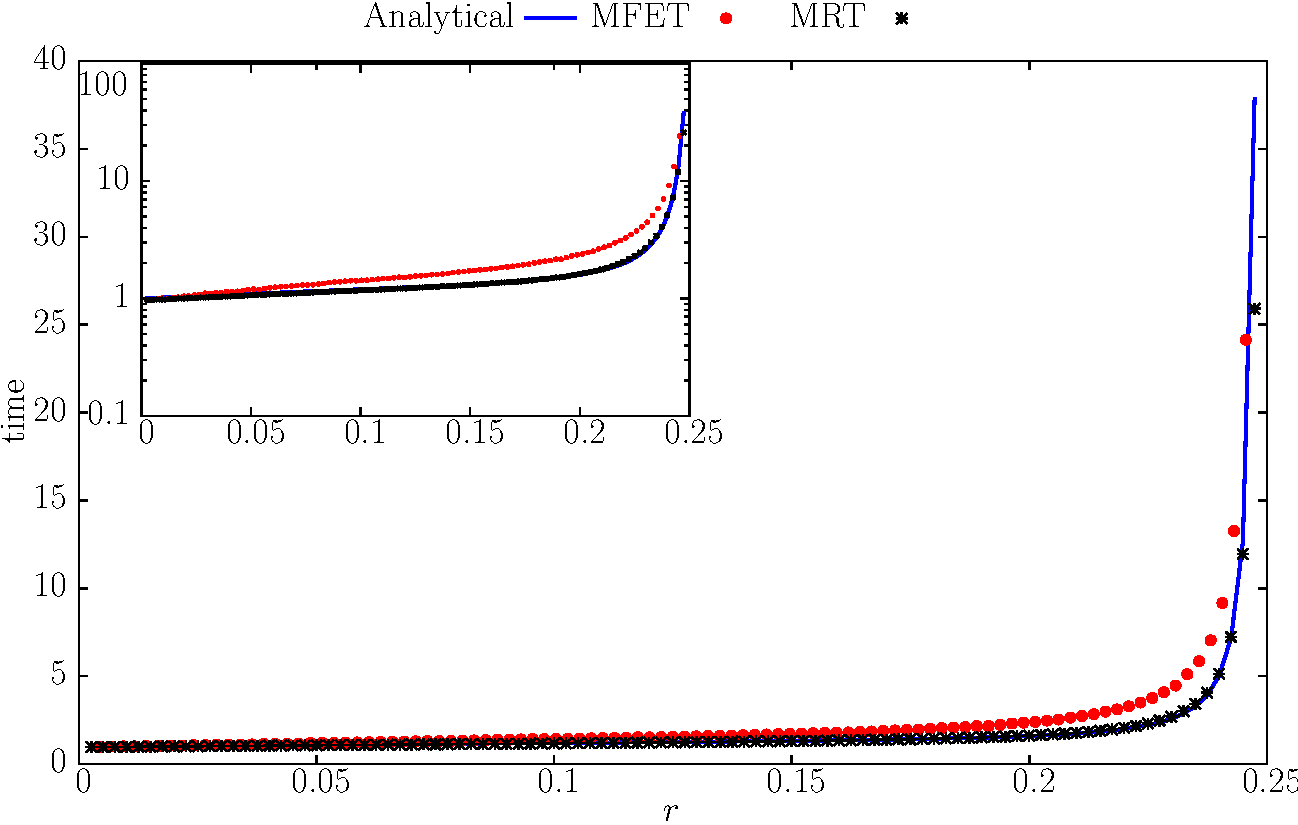
\includegraphics[width=0.45\textwidth]{./FigurasPerfectas/FistHopTime01-ForPaper.pdf}
  \caption{The mean first event time for the hopping event (MFET).
    We compare against the \emph{mean return time} (MRT), theoretical
and numerical. We observe how it is conterintuitivelly slightly longer,
but the qualitative behaviour is almost equal. A logarithmic inset
shows the behaviour across a wider range of scales. }\label{FirstHopp01}
\end{figure}cd

\begin{figure}[h]
  \centering
  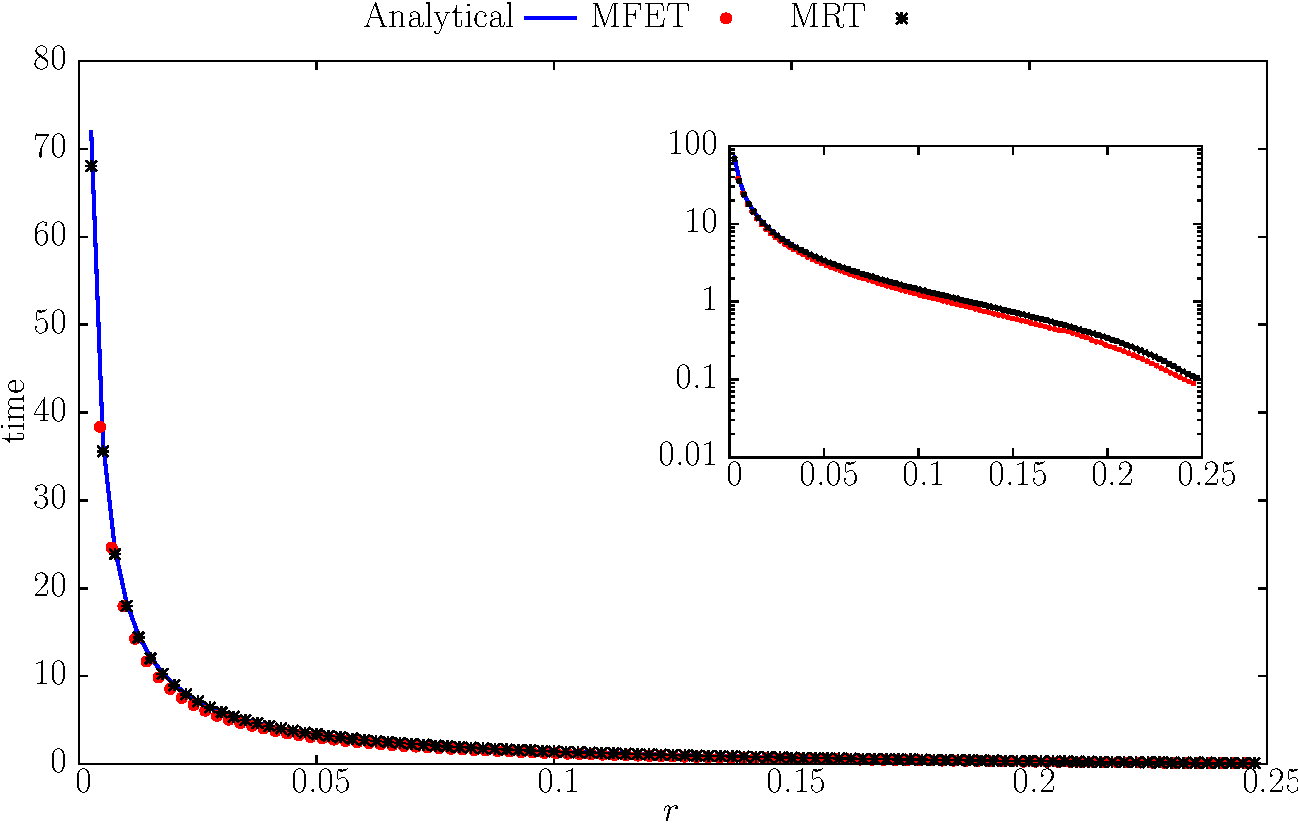
\includegraphics[width=0.45\textwidth]{./FigurasPerfectas/FistCollTime02-ForPaper.pdf}
  \caption{The mean first collision time as function of the radius.
    Here we have  a slighter shorter time as the radius increases. The difference
is more notorious on the semi-log plot in the inset. 
 }\label{FirstCol01}
\end{figure}

\begin{figure}[h]
  \centering
  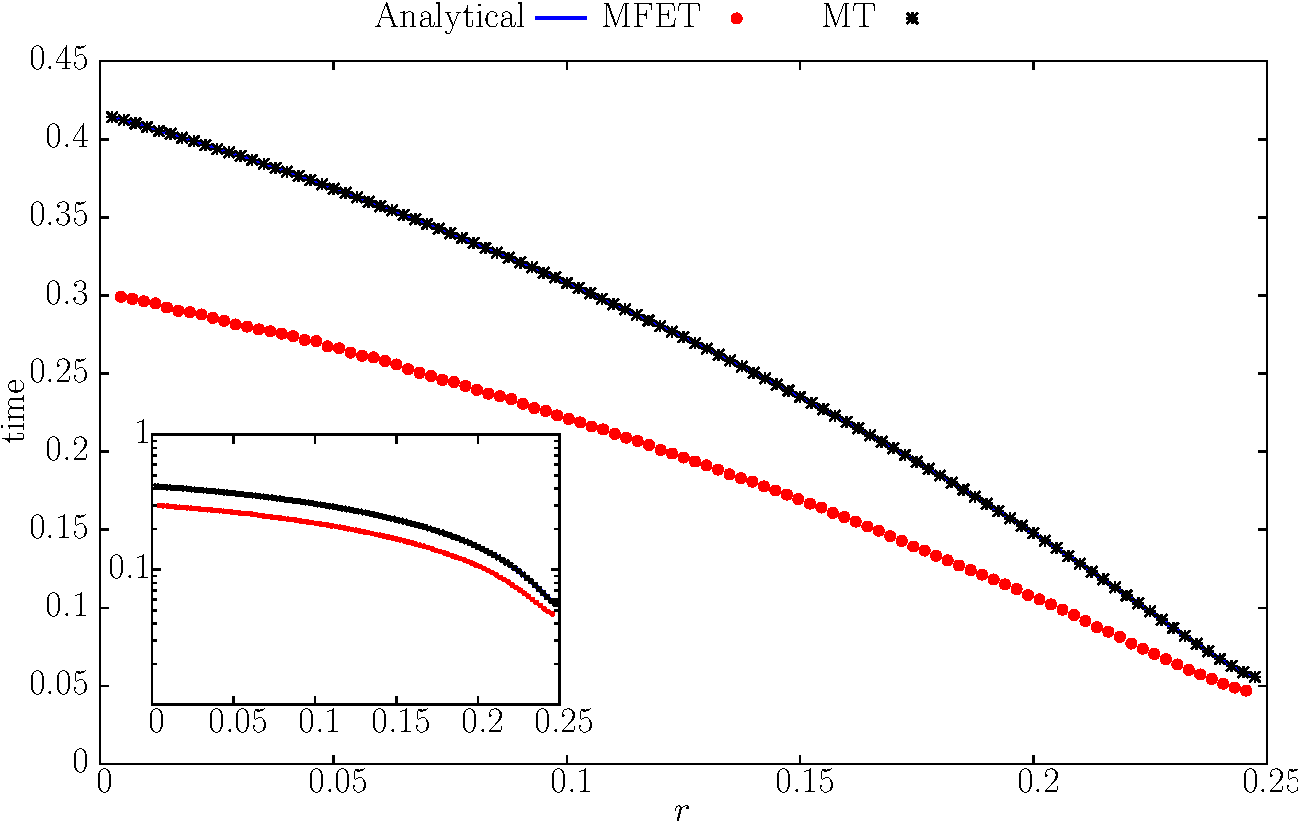
\includegraphics[width=0.45\textwidth]{./FigurasPerfectas/FistImpactTime01-ForPaper.pdf}
  \caption{The mean first impact-on-walls time as function of the radius. Again, 
    we observe the same qualitative behaviour but now the whole range is below
    the mean return time. This is to be expected, as for any initial condition
    we would have a past condition on the wall. For very
    large radius the step away from the wall is almost negligible.}\label{FirstImp01}.
\end{figure}


\section{Conclusions}


The model of two discs in a box has been extensively studied, and
very interesting results have been obtained which could help
to derive reaction
and diffusion times from basic underlying phenomena.  Here
we provide, for the first time, exact analytic expressions for the mean hopping and
collision times. 
%The 
%results which have helped us to do this came from the
%extensive theory of chaotic billiards. The subjacent theory
%of ergodic systems already contains strong theorems and formulas
%that only need judiciously application to show their 
%elucidating power. The step done by Machta and Zwanzig in
%that direction is a clear example of grounding that
%theory in applicable research. We have expanded
%that line by showing that other phenomena can be modeled
%as return times to appropriately chosen surfaces of section. 
The analytical results derived 
confirm the limiting behaviour obtained
by Bowles \etal by a different method, and Monte Carlo simulations confirm 
the results. 
Even though no exact expression is available for first event times, these follow
the same qualitative behaviour as the mean return times.

%The same technique can be further exploited for some other
%qualities simply by solving the adequate measures
%of volumes and areas. For Transport and Reaction problems
%the results that we have shown here could be made to serve
%the purpose of deriving the corresponding constants from first
%principles.

\appendix
\section{Area and volume calculations}
\label{app:area_volume}

\subsection{Volume}\label{VolApen}

We use the same notation as in the rest of the paper.
Do simplify the formulas, we do not write explicitly the dependence of $a$ and $b$ on $r$.

An implicit assumption was made on the limits of integration in \eqref{integraltotal}. If $w, h > 4r$, then the limits of integration
are unaffected by the radius of the circles.
In order to avoid uninteresting constant terms
in the formulas, we integrate
the excluded volume, instead of the available one. 

We begin the derivation after integrating out $X$ and $Y$:
\begin{equation}\label{VolumenGeneral}
V/16 =\iint \rd x \rd y \left[ 2ab-\sqrt{2}(ay+bx)+x y \right]
\indicator{x^2+y^2 < 2r^2 }.
\end{equation}
A diagram helps us visualize the limits of integration. The most general
case is (without loss of generality) $h < w < 2h$, so that, as the radius of the
discs increases, we can pass from the regime where both vertical and horizontal
hopping occur, to the one where only vertical hopping
is possible, to the one where no hopping is possible but a certain amount of movement
can still occur. The three regimes are characterized by the following inequalities:
\begin{itemize}
\item All hopping possible: $0<r \leq h/4$
\item Only vertical hopping possible: $h/4 < r \leq w/4$
\item No hopping possible: $w/4 < r < (h+w-\sqrt{2hw})/2$
\end{itemize}
The largest possible radius size is illustrated in figure~\ref{radiomaximo}.
\begin{figure}[h]
  \centering
  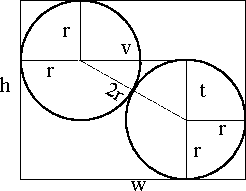
\includegraphics[width=0.4\textwidth]{FigurasPerfectas/DiagramaRadioMaximo.pdf}
  \caption{The largest possible radius for $h<w<2h$. From the diagram
    one can see that $t^2+v^2=(2r)^2$, $h=t+2r$ and $w=v+2r$, from which
    one can deduce the value for $r$.}
  \label{radiomaximo}
\end{figure}
We shall look at these regimes on the integration space. The first one is solved
on the main text, but we shall repeat it here with other coordinate system as to
make some points. In figure \ref{diaglimites} we present the three regimes as
the shaded area where we perform the integration. 
  
\begin{figure}[h]
        \centering
        \begin{subfigure}[b]{0.32\textwidth}
          \centering
          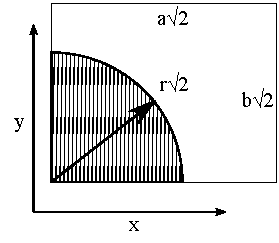
\includegraphics[width=\textwidth]{FigurasPerfectas/DiagramaIntegraCaso1.pdf}
          \caption{$r<b$}
          \label{Caso1}
        \end{subfigure}%
        ~ %add desired spacing between images, e. g. ~, \quad, \qquad etc.
        % (or a blank line to force the subfigure onto a new line)
        \begin{subfigure}[b]{0.32\textwidth}
          \centering
          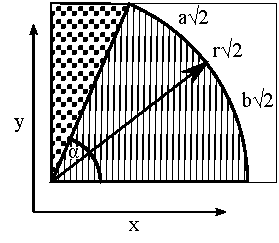
\includegraphics[width=\textwidth]{FigurasPerfectas/DiagramaIntegraCaso2.pdf}
          \caption{$b<r<a$}
          \label{Caso2}
        \end{subfigure}%
        ~ %add desired spacing between images, e. g. ~, \quad, \qquad etc.
          %(or a blank line to force the subfigure onto a new line)
        \begin{subfigure}[b]{0.32\textwidth}
          \centering
          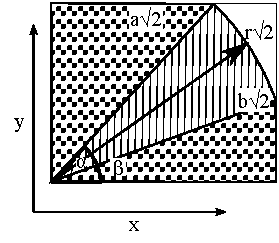
\includegraphics[width=\textwidth]{FigurasPerfectas/DiagramaIntegraCaso3.pdf}
          \caption{$a,b<r$}
          \label{Caso3}
        \end{subfigure}%
        \caption{The three possible cases. The shaded area is where the integral
          must be evaluated. In the first case all hopping is possible, the middle case
          only allows for vertical hopping and the last case excludes hopping but there
        is still possibility for the discs to fit inside the table.}
\label{CasosIntegra}
\end{figure}
The shaded area in figure \ref{CasosIntegra} represents where the indicator function
has value 1. We can translate that to well chosen limits of integration. Notice
how the hatched area in the first three cases may be integrated in polar coordinates
simplifying the three cases to three cases of evaluation. We shall call the
indefinite integral $V_h(r,\alpha,\beta)$ (h is for ``hatched'').
As can be seen from figure \ref{CasosIntegra}, the all hopping possible regime
means that $\alpha = \pi/2, \beta=0$, the vertical hopping regime is where
$\alpha < \pi/2, \beta=0$, and the no hopping regime is where $\pi/2 > \alpha > \beta > 0$.

\begin{equation}\label{Vhatch1}
\begin{split}
V_h(r,\alpha,\beta)/16 &=
\iint \rd x \rd y \left[ 2ab-\sqrt{2}(ay+bx)+x y \right]
\indicator{x^2 + y^2 < 2r^2}\\
&=
\iint \rd \rho \rd \theta \rho 
\left[ 2ab -\sqrt{2}(a\rho\sin\theta+b\rho\cos\theta) +\rho^2 \cos\theta\sin\theta \right]
\indicator{\rho^2<2r^2 }
\end{split}
\end{equation}
The integrator function becomes the limits over the $\rho$ integrating variable.
We set the $\alpha, \beta$ as the other two limits. The perform the
integral over the $\rho$ which doesn't change in the three regimes.
\begin{equation}
  \begin{split}
 V_h(r,\alpha,\beta)/16 &=\iint\limits_{\beta,0}^{\alpha,r\sqrt{2}} \rd \rho \rd \theta \rho (2ab
-\sqrt{2}(a\rho\sin\theta+b\rho\cos\theta)
+\rho^2 \cos\theta\sin\theta)\\
 &=\int\limits_\beta^{\alpha}  \rd \theta  
(2abr^2 - r^3 4/3 (a\sin\theta+b\cos\theta)+r^4 (\cos\theta\sin\theta))\\
\end{split}
  \end{equation}
Now we integrate over the $\theta$ variable:
\begin{equation}\label{Volrtheta}
  V_h(r,\alpha,\beta)/16 = 2r^2ab\theta+4/3*r^3(a\cos\theta-b\sin\theta)
  +\frac{r^4 \sin^2\theta}{2} \Bigg\vert_\beta^\alpha
\end{equation}
For the case in which all hopping is posible, the expression in eq. \ref{Volrtheta}
takes the values $\alpha=\pi/2, \beta=0$ and after multiplying by 16 both sides,
we recover the Munakata and Hu formula. For the other two cases, we can use the following
facts:
\begin{align}
  \sin\alpha&=b/r & \cos\beta&=a/r 
\end{align}
and the corresponding inverse relations and Pythagoric identities.
Then, in the case that all hopping is excluded, we end with the following beautiful
formula for excluded volume.
\begin{multline}\label{VolCaso3}
  V(r \vert r>w/4 )=32abr^2(\arcsin(b/r)-\arccos(a/r))\\
  +\frac{64r^3}{3}\biggl((a\sqrt{1-b^2/r^2}+b\sqrt{1-a^2/r^2})-(a^2+b^2)/r\biggr)\\
  +r^2/2(a^2+b^2-r^2)
\end{multline}

Now we treat the dotted areas in the figures \ref{Caso2} and \ref{Caso3}. Those are triangular
and are more easily treated in Cartesian coordinates. We start with the upper
triangular region, the subscript $ds$ indicating ``dotted superior'',
and show the procedure, and then we cite the result for the
other triangle.
First, we realize that as we are inside the triangle, the Characteristic function
translates so a simple integration limit:

\begin{equation}
  \begin{split}
    V_{ds}(r) /16 &=\iint \rd y \rd x [2ab-\sqrt{2}(ay+bx)+xy] \indicator{(x)^2+(y)^2<2r^2 }\\
    &=\int_0^{b\sqrt{2}}\rd y \int_{0}^{y\sqrt{r^2-b^2}/b} \rd x [2ab-\sqrt{2}(ay+bx)+xy] \\
   &=\int_0^{b\sqrt{2}}\rd y \bigl[2abx-\sqrt{2}(ayx+bx^2/2)+x^2y/2\bigr]_{0}^{y\sqrt{r^2-b^2}/b} \\
      &=\int_0^{b\sqrt{2}}\rd y
        \bigr[
          2aby\frac{\sqrt{r^2-b^2}}{b}
          -\sqrt{2}
          \bigr(
          \frac{ay^2\sqrt{r^2-b^2}}{b}
            +\frac{y^2(r^2-b^2)}{2b}
            \bigl)
           +\frac{y^3(r^2-b^2)}{2b^2}
           \bigl]\\
        &= \Bigr[ay^2\sqrt{r^2-b^2}-
          \frac{\sqrt{2}y^3}{3}
          \bigr(
          \frac{r^2-b^2+2a\sqrt{r^2-b^2}}{2b}
            \bigl)
            +\frac{y^4(r^2-b^2)}{8b^2}
            \Bigl]_0^{b\sqrt{2}}\\
          &=2ab^2\sqrt{r^2-b^2}
          -\frac{2b^2(r^2-b^2+2a\sqrt{r^2-b^2}}{3}+\frac{b^2(r^2-b^2)}{2}\\
          V_{ds}(r)&=32ab^2\sqrt{r^2-b^2} -\frac{32
            b^2}{3}(r^2-b^2+2a\sqrt{r^2-b^2}) +8b^2(r^2-b^2).
  \end{split}
  \end{equation}
The procedure is similar for the doted inferior region on fig. \ref{Caso3},
and gives a symmetric expression:
\begin{equation}
          V_{di}(r)=32a^2b\sqrt{r^2-a^2} -\frac{32
            a^2}{3}(r^2-a^2+2b\sqrt{r^2-a^2}) +8a^2(r^2-a^2).
\end{equation}

This expressions would account for all volume available in the configuration space, but
cannot be used for calculation of all event times that interest us. We need also
expressions that take into account that this space is divided in disjoint components,
as some events become impossible in each of these subsystems. As an example,
that will be detailed in the next section, disc 1 cannot hit the left wall if
it started on the right and horizontal hopping is excluded. So we have to
take into account that only half of the positions are available (due to symmetry)
and then take into account that in the formula in eq. \ref{meanfreetime}.

Due to the symmetry of the problem we can state that the available volume
for each disjoint component of the dynamical system is an equal fraction
of the total. For example, if horizontal hopping is no longer possible
($w/4<r<h/4$), there are two symmetric disjoint components: the dynamical system
that starts with disc 1 on the left and the one that starts with the disc 1 on
the right side. Both have to occupy the same phase space volume, as they are
symmetric under interchange of labels. If $(h<4\leq r$), then the system gets further
divided into four disjoint components. 



\subsection{Area}

The above procedure must be repeated for the different
area calculations. We use a Dirac delta to represent each touching
event. We multiply the characteristic function of the available space by the Dirac delta, and
then again divide it into the three cases, namely, all hopping, only vertical hopping
and no hopping possible, again referring to the figure \ref{CasosIntegra}.
Sometimes it turns out to be easier to obtain 
the integral  over all configuration space and then exclude the part that
corresponds to the overlapping condition. Again, the hatched area of the exclusion
condition has a simpler representation in polar coordinates, and the triangular
(dotted) regions can be treated in rectangular coordinates.



The areas representing different types of collision events require careful treatment of Dirac delta operators.
In general, an event is represented by a certain constraint of the form
$f(x_1, x_2 , y_1,y_2) =0 $; the measure of the corresponding three-dimensional manifold (surface) in configuration space is
\begin{equation}
  A_f=\iiiint \rd {x_1}  \rd {x_2}  \rd {y_1}  \rd {y_2} \delta(f(x_1, x_2 , y_1,y_2))
  \indicator{(x_1-x_2)^2+(y_1-y_2)^2>4r^2 }
\end{equation}
We must take into account that any change of coordinates inside the Dirac delta will include
a Jacobian factor for the volume element. 

Firstly
we integrate over the set $y_1 - y_2=0$ which happens to be different to the set
$y=0$ by a factor of $\sqrt{2}$ this is not obvious until one does the detailed calculations:
\begin{widetext}\label{ahopcart}
\begin{equation}
 A_\text{hopp} = \int \limits_{x_1 = -a}^a \rd {x_1} \int\limits_{x_2 = -a}^a \rd {x_2}
\int\limits_{y_1 = -b}^b \rd {y_1} \int\limits_{y_2 = -b}^b \rd {y_2} \, \indicator{ (x_1-x_2)^2 + (y_1-y_2)^2 \ge (2r)^2 } \delta(y_1-y_2).
\end{equation}
\end{widetext}
We have to acknowledge this: using Dirac Delta Operators does not grant us permission
to ignore multiplicative factors. As a simple example consider the following
development:
%\begin{equation}
  \begin{align*}
    \int f(x) \delta(a x) \rd x \\
    \text{ Let } y=ax \text{, then } \rd y = a \, \rd x\\
    \int f(y/a) \frac{\delta(y)}{a} \rd y 
  \end{align*}
 % \end{equation}
  Then we apply this to the expression in eq. \ref{ahopcart} and work the following
  derivation:
  \begin{align}
    A_\text{hopp}/16 & = \int_0^{a\sqrt{2}} \rd x  \int_0^{b \sqrt{2}} \rd y
    \int_0^{a\sqrt{2}-x} \rd X  \int_0^{b \sqrt{2}-y} \rd Y
    \indicator{x^2+y^2 \geq 2 r^2} \delta (y\sqrt{2})\\
    &= \frac{1}{\sqrt{2}} \int_0^{a\sqrt{2}} \rd x  \int_0^{b \sqrt{2}} \rd y
    (a\sqrt{2}-x)(b\sqrt{2}-y)
    \indicator{x^2+y^2 \geq 2 r^2} \delta (y)\\
    &=\frac{1}{\sqrt{2}} \int_0^{a\sqrt{2}} \rd x
    \indicator{x^2\geq 2 r^2} \\
    &=\frac{1}{\sqrt{2}} \int_{r\sqrt{2}}^{a\sqrt{2}} \rd x
    (2ab-xb\sqrt{2})\\
    &=\frac{1}{\sqrt{2}}\biggl[2abx-\frac{x^2b}{\sqrt{2}} \biggr]_{r\sqrt{2}}^{a\sqrt{2}}\\
      A_\text{hopp}&=16b(a-r)^2
  \end{align}  
  For other areas we take similar precautions. The area of collisions in
  the 4D configuration space is when $\sqrt{(x_1-x_2)^2+(y_1-y_2)^2}=2r$, so the
  expression for its size would be:
  \begin{equation}
    A_\text{col}=\iiiint _{-a,-a,-b,-b}^{a,a,bb,}
    \rd x_1 \rd x_2 \rd y_1 \rd y_2 
    \delta (\sqrt{(x_1-x_2)^2+(y_1-y_2)^2}-2r).
    \end{equation}
  Then we procede to juggle the expression inside the Dirac Delta operator:
  \begin{align}
    A_\text{col}/16 & =\iiiint _{0,0,0,0}^{a\sqrt{2},a\sqrt{2}-x,b\sqrt{2},b\sqrt{2}-y}
    \rd x \rd X \rd y \rd Y
    \delta (\sqrt{2x^2+2y^2}-2r)\\
    A_\text{col}/16 & =\iint _{0,0}^{a\sqrt{2},b\sqrt{2}}
    \rd x \rd y 
   \bigl[ 2ab-\sqrt{2}(ay+bx)+xy \bigr]
    \delta (\sqrt{2x^2+2y^2}-2r).
    \end{align}
  We change to polar coordinates as we did in \ref{VolApen}:
  \begin{align}
    x^2+y^2 =: \rho   \Rightarrow &  \delta(\sqrt{2x^2+2y^2}-2r) \rightarrow
    \delta(\sqrt{2}\rho-2r)   
    \end{align}
  Then we continue straightforwardly:
    \begin{align}
    A_\text{col}/4 & =\iint 
    \rd \theta \rd \rho \rho
    \bigl[2ab-\sqrt{2}\rho(a\sin\theta+b\cos\theta)+\rho^2\cos\theta\sin\theta
      \bigr]
    \delta(\sqrt{2}\rho-2r) \\
    &=\int_\beta^\alpha \rd \theta r
    \bigl[
      2ab-2r(a\sin\theta+b\cos\theta)+2r^2\cos\theta\sin\theta)
      \bigr] \\
    & = 2abr(\alpha-\beta) + 2r^2 [a (\cos \alpha-\cos\beta) -b (\sin\alpha -\sin\beta)]
    +r^3(\sin^2 \alpha -\sin^2\beta)
    \end{align}
    We have used the same trick as in previous subsection to obtain a general expression
    that works even when hopping is not possible. In the case of $r<w/4$ (all hopping possible)
    we have the substitution $\alpha=\pi/2$ and $b=0$, obtaining the result stated previously
    in eq. \ref{AreaChoque}. It is practical to leave here the expression for 1/4 of the
    total area. The symmetry of the cases makes it so that when the phase space splits
    into disjoint components, the volume accessible and the area accessible scale in
    the same manner.
    

    For a collision with the wall we apply again a Dirac Delta, and then a change
    of variables on the three surviving integrating coordinates. Once again, we
    have to be careful with the multiplicative factors that appear due to change
    of variables. Let us suppose that we want the area that represents hits of
    the disc 2 against the right wall. That means that $x_2-a=0$. 
    \begin{align}
      A_{x_2=a} & =\iiiint_{-a,-a,-b,-b}^{a,a,b,b} \rd x_1 \rd x_2 \rd y_1 \rd y_2 
      \indicator{(x_1-x_2)^2+(y_1-y_2)^2 \geq (2 r)^2} \delta (x_2-a)\\
      &=\iiint_{-a,-b,-b}^{a,b,b} \indicator{(x_1-a)^2+(y_1-y_2)^2 \geq (2 r)^2} 
    \end{align}
    Changing variables;
    \begin{equation}
      \frac{y_1-y_y}{\sqrt{2}} =  y  \qquad \frac{y_1+y_y}{\sqrt{2}}=Y \qquad \frac{x_1-a}{\sqrt{2}}=x
    \end{equation}
    Integrating over $x$,
    \begin{align}\label{areachoquexy}
      A_{x_2=a} & =\sqrt{2}\iiint_{-\sqrt{2}a,-\sqrt{2}b,-\sqrt{2}b+|y]}^{\sqrt{2}a,\sqrt{2}b,\sqrt{2}b-|y|}
        \rd x \rd y \rd Y 
      \indicator{(x^2+y^2 \geq 2 r^2} \\
      &=2\sqrt{2}\iint_{-\sqrt{2}a,-\sqrt{2}b}^{\sqrt{2}a,\sqrt{2}b}
        \rd x \rd y (\sqrt{2} b - |y|)
      \indicator{(x^2+y^2 \geq 2 r^2}
    \end{align}
    
    
    In the case that all hopping is possible there are no problems with the above derivations,
    but if vertical hopping is excluded, then there are differences.
    We must acknowledge some impossibles. If $r>h/4$, and the disc 2 starts
    on the left, it will never be able to hit the right wall. So, actually, this
    is a subsystem of the whole dynamic system in which our general formula needs
    to be adjusted. We can trace this problem to the original purpose of
    formula \ref{meanfreetime}
    was to find mean escape times. A particle cannot escape a volume if the exit is
    not in contact with that volume. So after hopping in one or both direction
    becomes impossible, the dynamical system gets split into disjoint components
    that never mix under the dynamics (ergodic components). So we have to take that
    into account. When $h/4<r<w/4$, a disk cannot interchange left-right positions,
    but can still move across all vertical available space.  After $r\geq w/4$,
    the system gets split again into more disjoint components and the
    area representing ``hitting the right wall'' is smaller (altough the probabilty is
    higher). So, when we calculate the ``avaible'' volume, we shall only use the
    part of the volume that belongs to the specific set that has a possibility of
    generating an event. We shall take into account what is written in the last
    paragraphs of the previous subsection. In this particular case, both the
    volume and area split into disjoint components with the same multiplicative
    factors, namely $1/2$ or $1/4$ of the total avaible. So this disapears in the
    result for mean times, but in the numeric, if we start with the discs in some
    prohibiting initial configuration, we may obtain the ``infinite time'' case.
    Taking that into account we wont integrate over the whole range, but only over
    the $1/4$ range, and then use the right multiplicative factor as needed.

    Again, it is simpler to evaluate the last expression in eq. \ref{areachoquexy}
    in the excluded space and then to subtract that from the whole configuration
    space evaluation.

    \begin{align}
      A_{x_2=a}/4 & =2\sqrt{2}\iint_{0,0}^{\sqrt{2}a,\sqrt{2}b}
        \rd x \rd y (\sqrt{2} b - y)
        \indicator{(x^2+y^2 \geq 2 r^2}\\
     &=\underbrace{2\sqrt{2}\iint_{0,0}^{\sqrt{2}a,\sqrt{2}b}
        \rd x \rd y (\sqrt{2} b - y)}_{\text{whole space}}
      -\underbrace{2\sqrt{2}\iint_{0,0}^{\sqrt{2}a,\sqrt{2}b}
        \rd x \rd y \rd Y 
        \indicator{(x^2+y^2 < 2 r^2}}_{\text{excluded space}}
       \end{align}
    The integrals are again routine to evaluate: the whole space part
    gives:
    \begin{equation}
      A_{\text{whole}}/4=16ab^2
    \end{equation}
    For the excluded part, we perform the same routine of evaluating the circular part
    in polar coordinates, and the triangular parts if they exists, in Cartesian.
    From the circular sector we get (see fig \ref{CasosIntegra} and the following explanation
    for $\alpha, \beta$ variables):
    \begin{equation}
      A_{sector}/4=16(r^2(\alpha-\beta)+2r^3/3(\cos\alpha - \cos\beta)
    \end{equation}
    The upper triangle where to give, for $\alpha \neq \pi/2$,
    \begin{equation}
    A_{ut}/4=\frac{4\sqrt{2}}{3}b^2\sqrt{r^2-b^2}
    \end{equation}
    And the lower triangle a similar expression with $a$ instead of $b$.

    Now, this are actually all the expressions needed for any collision, but
    to combine them and to use them meaningfully is still needed. For example,
    this last calculated area could be used as representation of the event of
    the disc 1 hitting the right wall, or the disc 2 hitting the left wall. Both
    can make sense in the case of excluded horizontal interchange. What would be
    the expression of any disk hitting the right wall? It would be twice this expression
    but only before the exclusion sets in. Then we need to take into account
    the disjointedness of the phase space and divide the cases accordingly.

    In the same vein we could conclude that the area that represents
    any collision (wall, discs, etc) can be obtained by summing all the other
    areas, before hopping is excluded. If there is some sort of hindrance to
    the movement, then the expression becomes different, again, a sum over
    disjoint components. This could lead to tedious exercises in cases ramifications.

    
    
    

    

    
\section{Acknowledgments}


DPS thanks Sidney Redner for asking the question that led to this work. The authors acknowledge financial support from grants CONACYT CB-101246 and CB-101997, and DGAPA-UNAM PAPIIT IN117117.





\bibliography{../../notasmixtas/TwoDiskBiblio}



\end{document}
